\section{Einleitung}
Der Einsatz von Robotern prägt zunehmend den Arbeitsmarkt und beeinflusst die Art und Weise wie Unternehmen ihre Prozesse gestalten. Diese Entwicklung beschränkt sich nicht nur auf klassische Einsatzgebiete wie die Industrie, in der beispielsweise Montageroboter eingesetzt werden, und den Verbrauchermarkt, in dem Staubsaugerroboter weit verbreitet sind, sondern zunehmened auch auf die Dienstleistungsbranche. So verzeichnete der Absatz von Service-Robotern für professionelle Anwendungen laut \ac{IFR} im Jahr 2022 einen Anstieg um 48\% \cite{IFR2023}, während der Absatz von Industrierobotern schwächer zunahm \cite[S.~9]{WorldRobotics2023} und von Service Robotern im Verbrauchermarkt sogar rückläufig war \cite[S.~37]{WorldRobotics2023}. Dieses Wachstum wird laut der \ac{IFR} durch eine gesteigerte Nachfrage getrieben, die unter anderem auf einen Mangel an Arbeitskräften zurückzuführen ist \cite[S.~33-34]{WorldRobotics2023}. Laut der \ac{BA} ist die Menge unbesetzter Arbeitsplätze in Deutschland in den letzten 10 Jahren um ~40\% gestiegen und - trotz des Rückgangs um ~18\% in den letzten zwei Jahren - weiter auf einem hohen Stand \cite{BA2024}. Insbesondere in der Gastronomie gibt es einen erheblichen Personalmangel, der zum Teil auf die Corona-Pandemie zurückzuführen ist, da in dieser Zeit viele Angestellte in andere Berufsfelder gewechselt sind. Laut dem Institut der deutschen Wirtschaft, welches sich auf Daten der \ac{BA} bezieht, sind während des Pandemiejahrs 2020 ~216.000 Arbeiter aus dem Gastgewerbe in ein anderes Berufsfeld gewechselt \cite[S.~1]{Jansen2022}. Service Roboter bieten durch eine effiziente Unterstützung des Personals die Möglichkeit den Personalmangel zu mitigieren. So ersetzen Service Roboter das Personal meistens nicht vollständig, sondern unterstützen es, sodass es mehr Zeit für andere Aufgaben wie die Kundenbetreuung hat \cite[S.~271-272]{Sprenger2015}. In der Gastronomie können Lieferroboter beispielsweise bestimmte Kellneraufgaben übernehmen und so das Personal entlasten.

\subsection{Hintergrund und Motivation}
In diesem Kontext hat sich die Firma Tobit Laboratories AG entschieden die Potenziale von Lieferrobotern für eigene Gastronomiestandorte zu erkunden. So hat das Unternehmen mehrere Lieferroboter von Pudu Robotics erworben, um diese Technologie zu testen. Zur Steuerung der Roboter aber auch zur Erweiterung der Funktionen wurde das \ac{BCB} entwickelt, das im Kapitel \ref{sec:BotControlBackend} näher erläutert wird. Die Roboter sollen zunächst im Firmengebäude für kleinere Botengänge eingesetzt werden. Abhängig der Ergebnisse könnten die Roboter dann möglicherweise in verschiedenen Gastronomiebetrieben eingesetzt werden. Hierfür müssen die Roboter zum einen auf verschiedene Aspekte, wie die Navigationsfähigkeit und Zuverlässligkeit geprüft werden. Zum anderen muss aber auch eine Anwendung entstehen, mit der die Roboter vor allem inutuitiv gesteuert, aber auch verwaltet werden können.

\subsection{Zielsetzung und Forschungsfrage}
Diese Arbeit setzt an diesem Punkt an und zielt darauf ab, eine Anwendung zu konzipieren und prototypisch zu implementieren, die die Steuerung und Verwaltung von Lieferrobotern ermöglicht und zudem eine Übersicht über deren Positionen bietet. Bei der Anwendung soll es sich um eine Webanwendung handeln, da diese im Gegensatz zu nativen Anwendungen eine plattformunabhängige Nutzung und sofortigen Verfügbarkeit ohne Download und Installation bieten. Für eine möglichst übersichtliche Darstellung der Roboterpositionen sollen 3D-Modelle der Gebäude genutzt werden in denen sich die Roboter befinden. Um eine reibungslose Integration der Roboter in Gastronomiebetriebe zu ermöglichen, sollte die Erstellung der 3D-Modelle mit minimalem Aufwand verbunden sein und möglichst unkompliziert sein. Hierbei gilt es zu beachten, dass die Erzeugung der 3D-Modelle nicht in der zu entwickelnden Anwendung integriert werden muss. Trotz des erhöhten Rechenaufwands, der mit der Darstellung von 3D-Modelle verbunden ist, soll die Anwendung außerdem performant sein.
% TODO Webanwendung Quelle

Aus dieser Zielsetzung ergibt sich die folgende Forschungsfrage: Wie kann eine effiziente und benutzerfreundliche Steuerung und Verwaltung von Servicerobotern implementiert werden?

\subsection{Methodik}
Die Forschungsfrage wird anhand des \ac{DSR} Ansatzes nach Hevner \cite{Hevner2004} beantwortet. Bei diesem handelt es sich um einen iterativen Forschungsansatz, mit dem Lösungen für praktische Probleme durch die Entwicklung von Artefakten gefunden werden. In dem Rahmen dieser Arbeit ist der zu entwickelnde Prototyp das Artefakt.

\subsubsection{Design Science Research nach Hevner}
Bei diesem Abschnitt handelt es sich um eine Zusammenfassung des \ac{DSR} Ansatzes nach Hevner \cite[S.~79-81]{Hevner2004}. Hevners Ansatz setzt sich aus drei Schleifen zusammen, wobei die Relevanz- und Strengeschleifen nur unterstützende Funktionen für die eigentliche Entwicklung - die Design-Schleife - bieten:

\begin{itemize}
    \item Die Relevanz-Schleife ergibt sich aus dem Verhältnis zwischen der Umgebung für die das Artefakt entwickelt wird und der Entwicklung des Artefakts. Aus den Menschen und Organisationen für die das Artefakt konzipiert wird und den Technologien die im Artefakt eingesetzt werden sollen ergibt sich die Umgebung. Aus dieser ergibt sich das Problem, das durch die Entwicklung des Artefakts gelöst werden soll. Für die Bewertung des Artefakts, wird dieses wiederum in der passenden Umgebung eingesetzt wird.
    \item Die Strenge-Schleife basiert auf der Wissensbasis, die zum einen aus dem Grundlagenwissen und Methodologien. Das Grundlagenwissen bietet eine Basis an Frameworks, Werkzeugen und Methoden mit denen das Artefakt entwickelt werden kann. Die Methodologien bieten eine Basis Methoden mit denen das Entwickelte Artefakt Ausgewertet werden kann. Durch die Entwicklung des Artefakts entsteht neues Wissen, das in der Wissensbasis ergänzt werden kann.
    \item In der Design-Schleife wird das Artefakt iterativ entwickelt. So wechselt sich das konstruieren und Auswerten des Artefakts regelmäßig ab, bis ein befriedigendes Ergebnis erreicht wurde.
\end{itemize}

In der Abbildung \ref{fig:DesignScienceResearch} wird dieser Prozess grafisch dargestellt. Man sieht die Relevanz- und Design-Schleifen als Unterstützungsprozesse für die eigentliche Forschung in der Form der Entwicklung des Artefakts.

\begin{figure}[H]
    \caption{Design Science Research nach Hevner}\label{fig:DesignScienceResearch}
    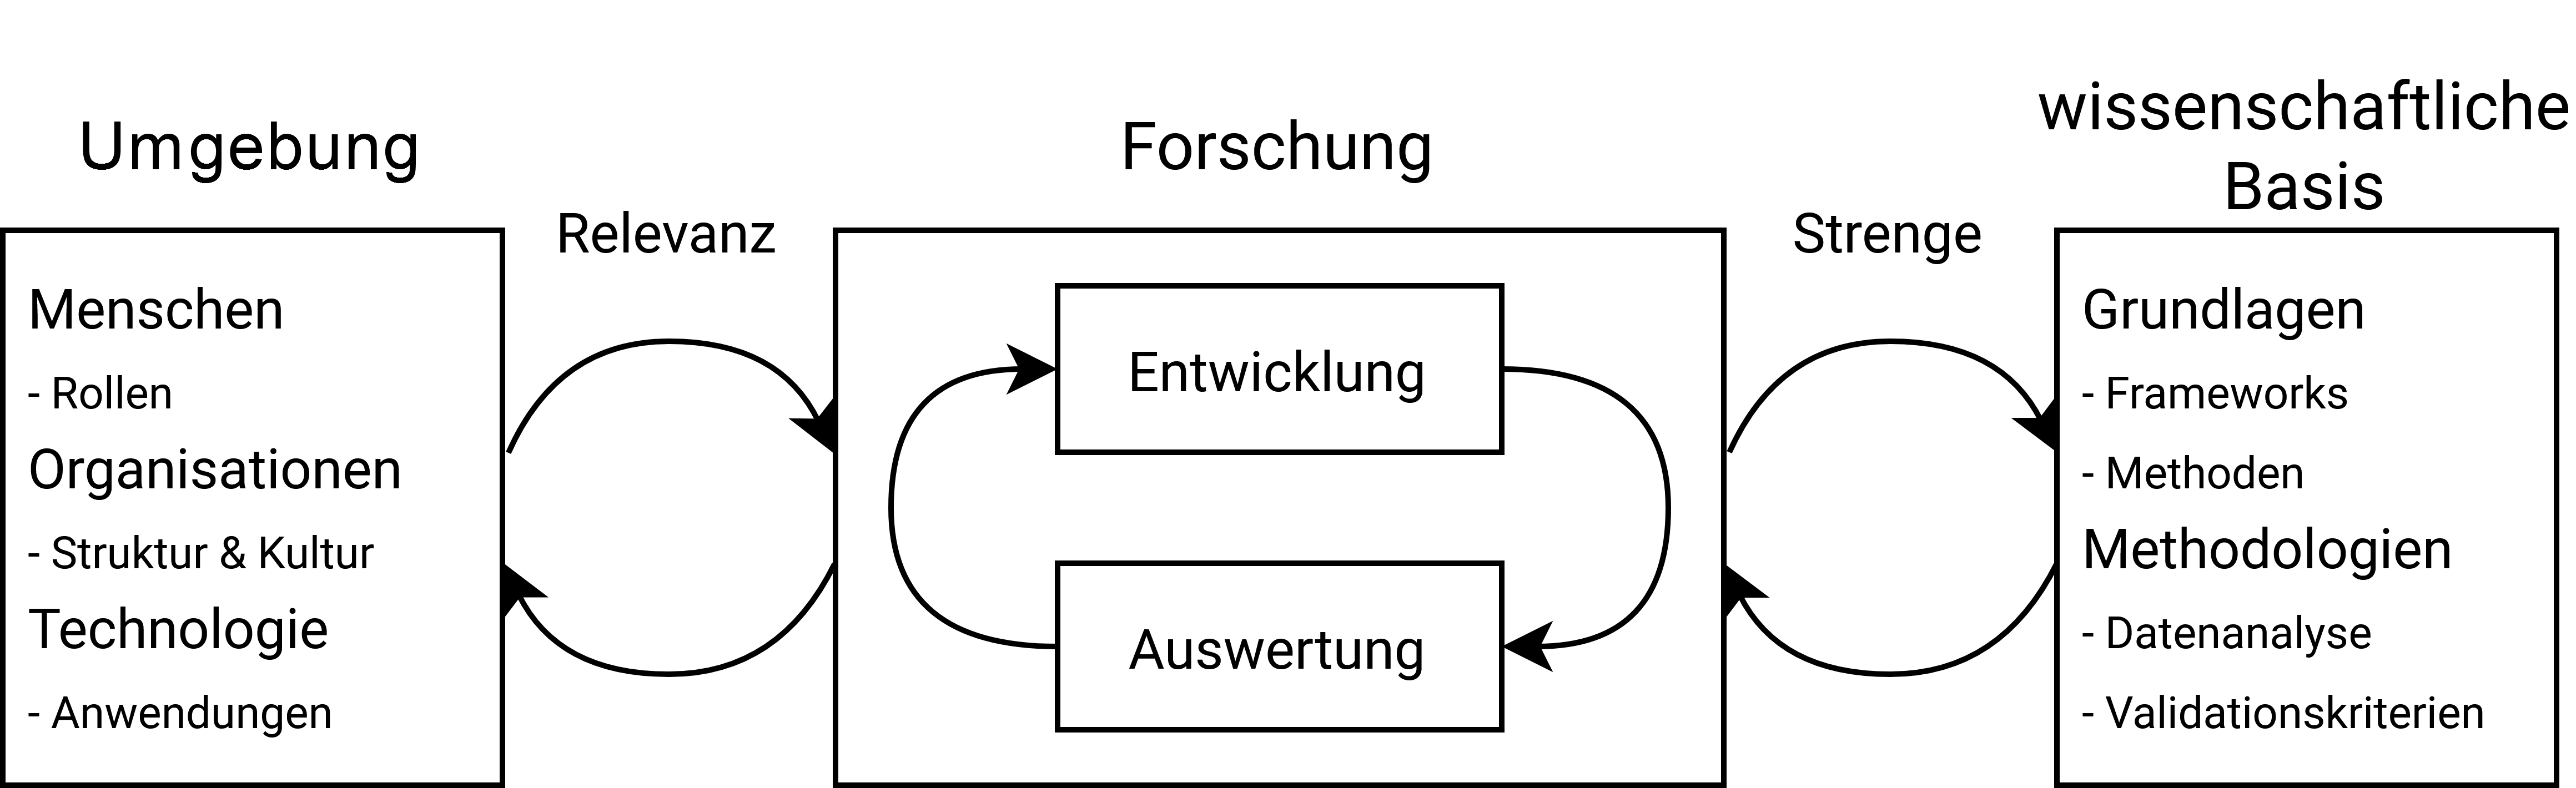
\includegraphics[width=0.9\textwidth]{Design Science Research.png}
    \\
    Quelle: In Anlehnung an Hevner et al. \cite[S.~80]{Hevner2004}
\end{figure}

\subsubsection{Design Science Research im Rahmen der Arbeit}

Die Prozesse des \ac{DSR} Ansatz nach Hevner werden in dieser Arbeit durch verschiedene wissenschaftliche Methoden abgebildet. Im ersten Schritt wird eine systematische Literaturrecherche durchgeführt mit der das grundlegende Verständnis über die Umgebung und die Basis an wissenschaftlichen Methoden geschaffen werden soll. So wird Wissen zu Service Robotern und zur Generierung von 3D-Modellen gesammelt. Auch wird Wissen zur wissenschaftlichen Auswertung von Software-Anwendungen gesammelt. Während der Implementierung des Prototyps weitet sich diese Literaturrecherche auf die Lösung von auftretenden Problemen aus. Die Umgebungsanforderungen werden nach der Wissensfindung über eine kurze Anforderungsanalyse definiert. Diese kann auf die funktionalen und nicht funktionalen Anforderungen aufgebaut werden, die sich bereits aus der Zielsetzung und der Formulierung der Forschungsfrage ergeben. So stehen die Anforderungen, dass der Prototyp eine Webanwendung sein und eine dreidimensionale Visualisierung bieten soll bereits fest. Auch steht bereits fest, dass der Prototyp benutzerfreundlich und effizient sein soll. Die Implementierung des Prototyps soll im Verfahren des Rapid Prototypings durchgeführt werden. So wechseln sich die Entwicklung und Auswertung der benutzerfreundlickeit und effizienz iterativ ab bis ein Prototyp entstanden ist, der die definierten Anforderungen erfüllt.
% TODO Quelle Rapid Prototyping
